\documentclass{instrukcja}        
\usepackage[polish]{babel}
\usepackage[utf8]{inputenc}
\usepackage[OT4]{fontenc}

\begin{document}
\materialnumber{5}
\course[Info I]{Informatyka I}
\material[Lab 5]{Instrukcja 5}
\author{W. Regulski}
\materialtitle

\section*{Tablice}
Celem zajęć jest wprowadzenie do używania tablic w języku C. Tablicą (ang. {\it array}) nazywamy ciąg zmiennych zgromadzony pod jedną globalną nazwą, które są identyfikowane indeksami. 
Na tych zajęciach zajmiemy się tylko tablicami statycznymi tzn. takimi, których rozmiar jest określany w momencie deklaracji\footnote{bardziej zaawansowany mechanizm alokacji tablic będzie tematem następnych zajęć}.
Tablicę statyczną deklarujemy tak, jak zwykłą zmienną, przy czym dodatkowo określamy jej długość. Wszystko wygląda, jak w przykładowym kodzie poniżej:

\begin{verbatim}
      double a[4];    	// deklaracja tablicy

      a[0] = 5.5;		   // przypisanie wartości do zmiennych
      a[1] = 3.521;
      a[2] = 6.45;
      a[3] = 4.51;

\end{verbatim}
Zwróć uwagę, że elementy tablicy sa indeksowane od \(0\) do \(n-1\), gdzie \(n\) to rozmiar tablicy. Można również zainicjalizować wszystkie elementy tablicy natychmiast (taki mechanizm jest użyteczny, jeśli wektory są stosunkowo krótkie):
\begin{verbatim}
     double b[3] = { 1.2, 2.4, -4.3};
\end{verbatim}
\section*{Piłki}

Zadanie polegać będzie na wygenerowaniu zestawu piłek w oknie graficznym oraz na wyszukiwaniu i określaniu ich specyficznych cech, jak np. minimalna, średnia i maksymalna pozycja, maksymanla masa itp. Przykładowy zbiór takich piłek jest widoczny na Rysunku 1.
\begin{figure}
\centering
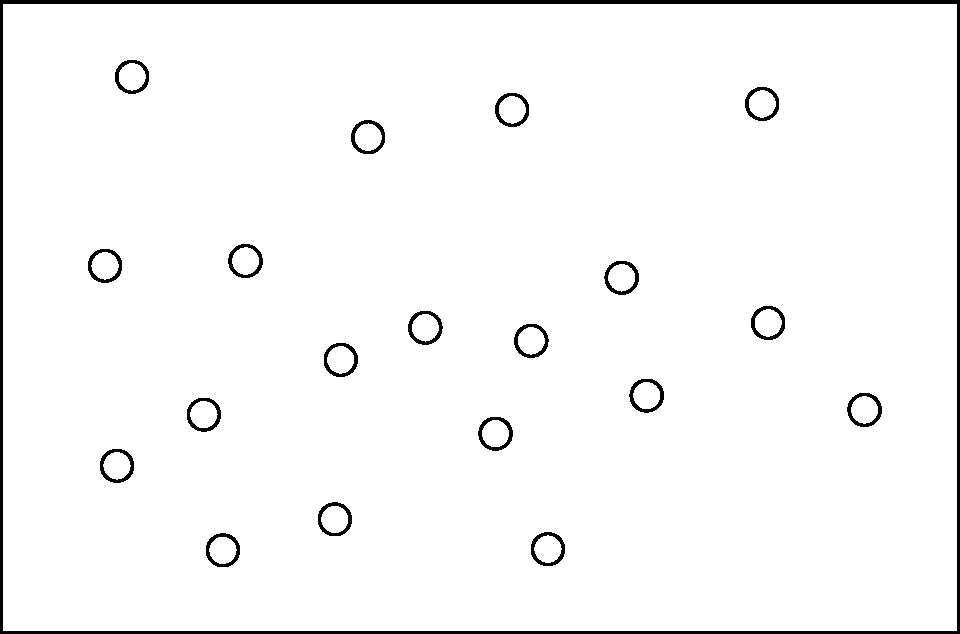
\includegraphics[width=0.3\textwidth]{kolka.pdf}

\caption{Piłki w ramce.}
\end{figure}
\section {Inicjalizacja}
Nasze piłki będą przychowywane tylko jako zestawy współrzędnych, ich prędkości oraz masy. Gdy będziemy chcieli obejrzeć piłki w oknie graficznym, po prostu użyjemy funkcji {\tt circle}. Toteż w symulacji będą potrzebne następujące wektory\footnote{tablice często będziemy nazywać wektorami, ze względu na fakt, że określenie "tablica" kojarzy się z obiektem o większej ilości wymiarów np. z macierzą}:
\begin{verbatim} 

double x[10],y[10];            // współrzędne piłek
double vx[10], vy[10];         // składowe prędkości piłek
double m[10];                 //masy piłek
\end{verbatim}

\subsection* {Pętla {\tt for}}

Większość operacji na tych zmiennych będziemy wykonywać, używając funkcji, które będą przyjmować wprowadzone wyżej wektory jako argumenty. Funkcje będą musiały mieć podaną długość wektorów tak, aby można było wykonać pewne operacje dla każdego z elementów tego wektora.
Jeśli chcemy np. zainicjalizować wszystkie współrzędne wartością \(0\), piszemy funkcję następującej treści:

\begin{verbatim}
void init(double *x, double *y, int N){

      for ( int i=0; i < N; ++i){
          x[i] = 0.0;
          y[i] = 0.0;}
}
\end{verbatim}



Wykorzystaliśmy tutaj pętlę {\tt for}, która pobiera 3 argumenty:
\begin{itemize}
\item wartość startową,
\item warunek działania (pętla działa, dopóki warunek \(i<N\) jest spełniony),
\item operację na argumencie (tutaj zwiększamy \(i\) o 1, co będzie najpowszechniejszą praktyką\footnote{Teoretycznie możemy w tym miejscu wykonać dowolną operację, jednak dla czytelności kodu zazwyczaj zwiększamy licznik pętli})
\end{itemize}

Taką funkcję wywołujemy w programie głównym, podając nazwy wektorów, na których ma ona działać oraz długość tych wektorów:

\begin{verbatim}

	init(x, y, 10);

\end{verbatim}

Zauważmy, że funkcja {\tt init} pobiera 2 wskaźniki do wektorów({\tt x} oraz {\tt y}) oraz jedną wartość (10). Dzięki temu funkcja operuje bezpośrednio na wektorach, na których ma operować i niczego nie musi zwracać\footnote{Zasady działania na wskaźnikach opisano w Instrukcji 4.2.}. 

\subsection*{Uwaga}
Ponieważ {\tt x} oraz {\tt y} są wskaźnikami do pierwszych elementów tablic, można użyć mechanizmu wyłuskania wartości ze wskaźników i iterować się po wskaźnikach. Poniższy fragment kodu pokazuje dwa równoważne sposoby dostępu do wartości z tablicy:

\begin{verbatim}
double a[3];
// po wartościach:
a[0] = 1.2;         a[1] = 3.13;         a[2] = 0.22;
//albo na wskaźnikach:
*(a)   = 1.2;           *(a+1) = 3.13;        *(a+2) = 0.22;
\end{verbatim}

\subsection*{Ćwiczenia}
Przed wykonaniem ćwiczeń upewnij się, że załączono bibliotekę \verb|winbgi2.h|, gdyż będziemy korzystać z grafiki.
\begin{enumerate}
\item Zadeklaruj wymienione wyżej wektory położeń, prędkości oraz mas. Utwórz 20 piłek.
\item Zadeklaruj okno graficzne o wymiarach \(Lx \times Ly\).
\item Napisz funkcję {\tt init(double *x, double *y, double *vx, double *vy)}, która wylosuje współrzędne położeń początkowych tak, aby powstałe piłki mieściły się w oknie graficznym a składowe prędkosci zawierały się w przedziale \(\langle-20,20\rangle\). Użyj funkcji \verb|rand()| znanej z poprzednich zajęć.
\item Wypisz na ekran współrzędne wszytkich piłek oraz ich prędkości.
\item Napisz funkcję {\tt display(double *x, double *y, int N)}, która wyświetli położenie i prędkości piłek. Wyświetl piłki.
\item Każdej piłce przypisz masę - niech piłka o indeksie \(i\) ma masę \(m_i=2i^2 + 1\).
\end{enumerate}

\section{Analiza położeń i mas}

Często nasz zestaw danych musimy poddać jakiejś analizie. Np. chcielibyśmy wiedzieć, która piłka ma największą współrzędną \(y\). W tym celu musimy dokonać przeszukiwania w danym zbiorze danych. Ponadto chcielibyśmy wykonać taką operację możliwie niskim kosztem. W tym przypadku możemy zrobić to, iterując się tylko raz po całym zbiorze piłeczek. Dodatkowo utworzymy tylko tymczasową zmienną (bufor), która będzie przechowywać maksymalna wartość współrzędnej \(y\). Ten bufor nazwiemy {\tt ymax }, gdyż po działaniu pętli to w nim zostanie wartość maksymalna. To wszystko ilustruje poniższy kawałek kodu:

\begin{verbatim}
double ymax=0.0;	//od czegoś trzeba zacząć

for( i=0; i < N; ++i){
     if(y[i] > ymax){
          ymax=y[i];}
}
\end{verbatim}

Powyższa pętla kroczy po wszystkich współrzędnych \(y\) i jeśli któraś z nich jest większa od wartości aktualnie znajdującej się w buforze, jej  \(y\) staje się nowym maksimum. Nie trudno zauważyć, że jeden taki cykl załatwia sprawę do końca. Oczywiście w tej samej pętli moglibyśmy zrobić inne interesujące nas rzeczy. Np. możemy zabrać się za liczenie średniej masy piłek:

\begin{verbatim}
double m_avg = 0.0;;

for( i=0; i < N; ++i){
         m_avg+=m[i];	//liczymy całkowitą masę piłek
}

m_avg = m_ang/N; //liczymy średnią
\end{verbatim}
	

\subsection*{Ćwiczenia}

\begin{enumerate}
\item Napisz fragment kodu, który znajduje piłki o minimalnej i maksymalnej współrzędnej \(x\) oraz \(y\). Na ekranie wypisz te minima i maksima wraz z indeksami tych piłek.
\item Napisz funkcję {\tt crossOut(double *x, double *y, int i)}, która przekreśli krzyżykiem piłkę o indeksie \(i\). Do skreślania użyj dwóch funkcji {\tt line}. Za pomocą tej funkcji skreśl piłki z poprzedniego podpunktu. 

\item Napisz fragment kodu, który policzy minimalną, średnią i maksymalną energię kinetyczną piłek. Wypisz te wartosci na ekran.
Energię kinetyczną liczymy ze wzoru \(E_k=1/2m(v_x^2+v_y^2)\). 
\item Na środku ekranu narysuj koło o promieniu równym \(0.3\) przekątnej okna graficznego. Następnie wykreśl wszystkie piłki, których środki nie znajdują się w obszarze tego koła.
\item Napisz funkcje {\tt swapX} i {\tt swapY}, które zamienią wskazane współrzędne piłek w zbiorze wg schematu pierwsza z ostatnią, druga z przedostatnią itd. Zamiana powinna odbyć się w obrębie jednej petli! Wyświetl nowy zbiór piłek po każdej zamianie.
\end{enumerate}

\section{*Zaawansowane przeszukiwanie}
Do tej pory mieliśmy do czynienia z iteracjami, których liczba rosła liniowo (tzn. proporcjonalnie) do rozmiaru zbioru. Co gdybyśmy chcieli np. porównywać piłki między sobą? Wówczas musielibyśmy iterować się po wszystkich parach piłek. Np. jeśli piłek jest 10, par jest 45. Taki proces ma koszt kwadratowy (dokładnie \(n(n-1)/2 \)). W poniższym przykładzie znaleźć maksymalną odległość między dwoma piłkami. Odległość między dwoma piłkami będzie dana wzorem: 
\begin{displaymath}
L=\sqrt{(x_{i}-x_{j})^2 +(y_{i}-y_{j})^2 }
\end{displaymath}
W najprotszej wersji możemy najpierw stworzyć tablicę, która przechowa wszystkie możliwe odległości, a następnie znaleźć jej maksimum. Jednak należy zrobić to bardziej elgancko, bez deklarowania dodatkowych tablic. Załatwi to następujący kod:

\begin{verbatim}
double L_max=0.0;
double L_tmp;        //dodatkowa zmienna dla czytelności kodu

for(i =0; i < 10; +i){
     for(j=i+1; j < 10; ++j){
          L = sqrt((x[i]-x[j])*(x[i]-x[j]) 
                  + (y[i]-y[j])* (y[i]-y[j]));
          if(L>L_max){
                   L_max = L;}
          }
}

\end{verbatim}
Zauważmy, że podpętla po indeksie \(j\) ma zakres zależny od  \(i\): nie ma sensu przeszukiwać wszystkich piłek wstecz. Wystarczy, że każda piłka o indeksie \(i\) policzy swoją odległość do piłek, których indeksy następują po niej samej.

\subsection*{Ćwiczenia}
\begin{enumerate}
\item Znajdź najmniejszą i najwiekszą odległość między piłkami. Wypisz te odległości oraz indeksy tych piłek na ekran.
\item Narysuj linie łączące 2 najbliższe piłki i 2 najdalsze.
\item Połącz liniami piłki, które są od siebie dalej niż \( Lx/2\).

\end{enumerate}




\end{document}
